%Pakete;
%A4, Report, 12pt
\documentclass[ngerman,a4paper,12pt]{scrreprt}
\usepackage[a4paper, right=20mm, left=20mm,top=30mm, bottom=30mm, marginparsep=5mm, marginparwidth=5mm, headheight=7mm, headsep=15mm,footskip=15mm]{geometry}

%Papierausrichtungen
\usepackage{pdflscape}
\usepackage{lscape}

%Deutsche Umlaute, Schriftart, Deutsche Bezeichnungen
\usepackage[utf8]{inputenc}
\usepackage[T1]{fontenc}
\usepackage[ngerman]{babel}

%quellcode
\usepackage{listings}

%tabellen
\usepackage{tabularx}

%listen und aufzählungen
\usepackage{paralist}

%farben
\usepackage[svgnames,table,hyperref]{xcolor}

%symbole
\usepackage{latexsym,textcomp}
\usepackage{amssymb}

%font
\usepackage{helvet}
\renewcommand{\familydefault}{\sfdefault}

%Abkürzungsverzeichnisse
\usepackage[printonlyused]{acronym}

%Bilder
\usepackage{graphicx} %Bilder
\usepackage{float}	  %"Floating" Objects, Bilder, Tabellen...
\usepackage[space]{grffile} %Leerzechen Problem bei includegraphics
\usepackage{wallpaper} %Seitenhintergrund setzen
\usepackage{transparent} %Transparenz

%for
\usepackage{forloop}
\usepackage{ifthen}

%Dokumenteigenschaften
\title{Summary CN1}
\author{Tobias Blaser}
\date{\today{}, Uster}


%Kopf- /Fusszeile
\usepackage{fancyhdr}
\usepackage{lastpage}

\pagestyle{fancy}
	\fancyhf{} %alle Kopf- und Fußzeilenfelder bereinigen
	\renewcommand{\headrulewidth}{0pt} %obere Trennlinie
	\fancyfoot[L]{\jobname} %Fusszeile links
	\fancyfoot[C]{Seite \thepage/\pageref{LastPage}} %Fusszeile mitte
	\fancyfoot[R]{\today{}} %Fusszeile rechts
	\renewcommand{\footrulewidth}{0.4pt} %untere Trennlinie

%Kopf-/ Fusszeile auf chapter page
\fancypagestyle{plain} {
	\fancyhf{} %alle Kopf- und Fußzeilenfelder bereinigen
	\renewcommand{\headrulewidth}{0pt} %obere Trennlinie
	\fancyfoot[L]{\jobname} %Fusszeile links
	\fancyfoot[C]{Seite \thepage/\pageref{LastPage}} %Fusszeile mitte
	\fancyfoot[R]{\today{}} %Fusszeile rechts
	\renewcommand{\footrulewidth}{0.4pt} %untere Trennlinie
}

\usepackage{changepage}

% Abkürzungen für Kapitel, Titel und Listen
%listen und aufzählungen
\usepackage{paralist}
\usepackage{mdwlist}

% list short cuts
\newcommand{\ul}{
	\begin{itemize}
}
\newcommand{\ulE}{
	\end{itemize}
}
\newcommand{\ol}{
	\begin{enumerate}
}
\newcommand{\olR}{
	\resume{enumerate}
}
\newcommand{\olE}{
	\end{enumerate}
}
\newcommand{\olS}{
	\suspend{enumerate}
}
\newcommand{\li}{
	\item
}
\newcommand{\dl}{
	\begin{description}
}
\newcommand{\di}[1]{
	\item[#1]
}
\newcommand{\dlE}{
	\end{description}
}
\newcommand{\ra}{
	$\rightarrow$
}

% chapter and section shortcuts
\newcommand{\ch}[1]{
	\chapter{#1}
}
\newcommand{\se}[1]{
	\section{#1}
}
\newcommand{\sse}[1]{
	\subsection{#1}
}
\newcommand{\sss}[1]{
	\subsubsection{#1}
}

\newcommand{\important}[1]{
	 \fcolorbox{black}{black}{ %
		\parbox{17cm}{%
			\vspace{0.1cm}
			\hspace{0.1cm}
   			\transparent{1.0}
			\color{white}
			\fontsize{12}{14} \selectfont #1
			\vspace{0.1cm}
   		}
    }
}

\newcommand{\expl}[2]{
	 \fcolorbox{gray}{gray}{ %
		\parbox{17cm}{%
			\vspace{0.1cm}
			\hspace{0.1cm}
   			\transparent{1.0}
			\color{white}
			\fontsize{12}{14} \selectfont 
			\textbf{Erklärung #1:} #2
			\vspace{0.1cm}
   		}
    }
}

\newcommand{\examp}[2]{
	 \fcolorbox{blue}{blue}{ %
		\parbox{17cm}{%
			\vspace{0.1cm}
			\hspace{0.1cm}
   			\transparent{1.0}
			\color{white}
			\fontsize{12}{14} \selectfont 
			\textbf{Beispiel (e) #1:} #2
			\vspace{0.1cm}
   		}
    }
}

\newcommand{\exam}[1]{
	 \fcolorbox{orange}{orange}{ %
		\parbox{17cm}{%
			\vspace{0.1cm}
			\hspace{0.1cm}
   			\transparent{1.0}
			\color{white}
			\fontsize{12}{14} \selectfont 
			\textbf{Prüfung:} #1
			\vspace{0.1cm}
   		}
    }
}

\newcommand{\definition}[2]{
	 \fcolorbox{teal}{teal}{ %
		\parbox{17cm}{%
			\vspace{0.1cm}
			\hspace{0.1cm}
   			\transparent{1.0}
			\color{white}
			\fontsize{12}{14}	
				\selectfont 
			\textbf{Definition #1:} #2
			\vspace{0.1cm}
   		}
    }
}


%links, verlinktes Inhaltsverzeichnis, PDF Inhaltsverzeichnis
\usepackage[bookmarks=true,
bookmarksopen=true,
bookmarksnumbered=true,
breaklinks=true,
colorlinks=true,
linkcolor=black,
anchorcolor=black,
citecolor=black,
filecolor=black,
menucolor=black,
pagecolor=black,
urlcolor=black
]{hyperref} % Paket muss unbedingt als letzes eingebunden werden!

\usepackage{graphicx}
\begin{document}

% Inhaltsverzeichnis
\tableofcontents
\clearpage


\ch{VLANs \& Campus Design}
\se{VLANs}
\expl{VLAN}{a VLAN = a Broadcast Domain = a Logical Network}

\sse{Vorteile}
\ul
	\li Arbeitsgruppen können über das gesammte Gelände verstreut sein
	\li Das Netzwerk ist flexibel und kann gut erweitert werden ohne die physische verdrahtung zu ändern
	\li Benutzer können in der gleichen Arbeitsgruppe bleiben, egal wo sie auf dem Gelände arbeiten.
	\li Jedes VLAN ist eine eigene Broadcast Domäne
\ulE
\expl{Switch}{Switch determiniert Physical Layer, Broadcast jedoch nicht}
\begin{figure}[H]
	\centering
	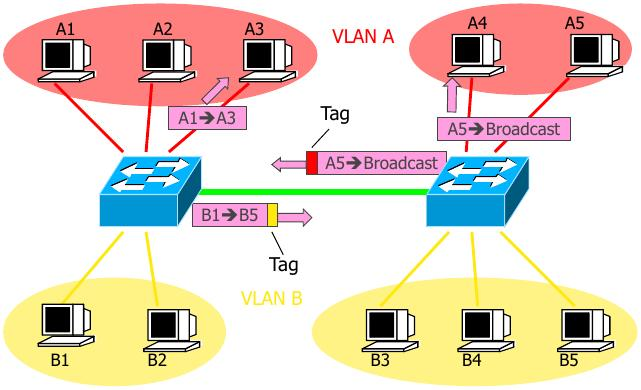
\includegraphics[scale=1.00]{img/V5.1.jpg}
	\caption{Virtual Lan's mit Paketen mit Tags}
	\label{}
\end{figure}
\ul
	\li Trennung der Broadcast Domäne
	\li Pakete erhalten Tag zur Zuordnung
\ulE

\sse{Tag}
\begin{figure}[H]
	\centering
	 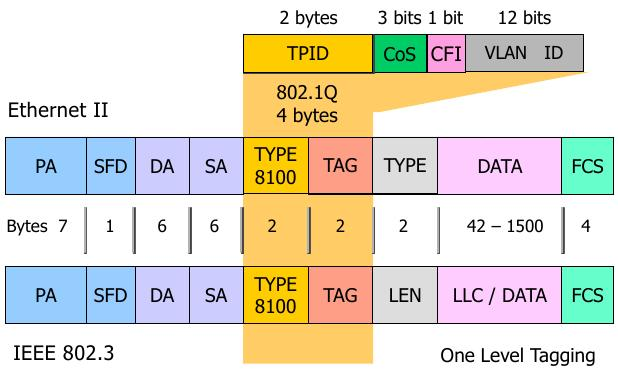
\includegraphics[width=\textwidth]{img/V5.2.jpg}
	\caption{Tagging Format}
	\label{}
\end{figure}
Vor dem Type Field wird ein weiteres Type Field und ein Tag Field eingefügt.

\sse{Kommunikation zwischen VLAN}
\ul
	\li VLAN sind untereinandern nicht erreichbar.
	\li Zur Verbindung wird ein Router benötigt.
	\li Der Router muss Routing anhand des Tags unterstützen, ansonsten muss mit den einzelnen irtuellen Netzen einzeln auf einzelne Ports gefahren werden.
\ulE
\begin{figure}[H]
	\centering
	 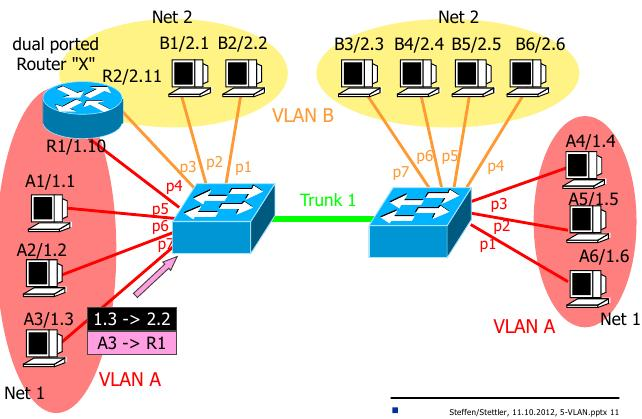
\includegraphics[width=\textwidth]{img/V5.3.jpg}
	\caption{Inter VLAN Trafic}
	\label{}
\end{figure}
\ol
	\li Multicast geht an Default Gateway (Router) weil es eine externe Adresse ist
	\li Switch kann Paket nicht in anderes VLAN senden
	\li Router bildet das MacPaket neu und schickt das Paket wieder los
	\li Der Switch switcht das Paket ins Net2 zum entsprechenden Host	
\olE
\expl{IP Paket}{Das IP Paket mit den globalen Adressen bleibt bestehen und wird vom Switch nicht verändert. Der Switch setzt nur den Tag.}

\sse{Transport über Layer2 Grenzen hinweg}
\begin{figure}[H]
	\centering
	 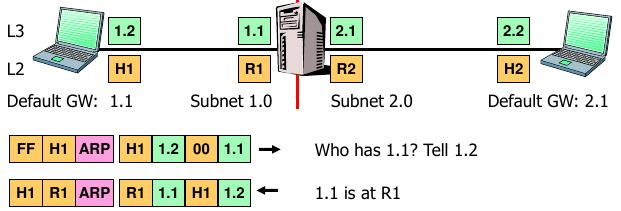
\includegraphics[width=\textwidth]{img/V5.4.jpg}
	\caption{}
	\label{}
\end{figure}
\begin{figure}[H]
	\centering
	 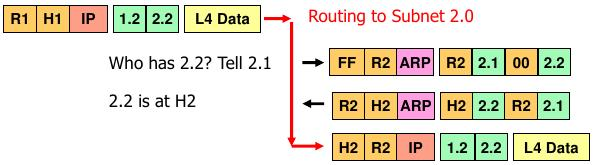
\includegraphics[width=\textwidth]{img/V5.5.jpg}
	\caption{IP Paket von Host 1.2 zu 2.2 senden}
	\label{}
\end{figure}
\definition{Default Gateway}{Alle Pakete, die nicht in mein Subnetz gehören, werden dorthin gesendet}
\ol
	\li ARP Broadcast \ra fragt nach Hardwareadresse von IP 1.1
	\li Default Gateway antwortet
	\li 1.2 Baut Paket zusammen und sendet es an den Default Gateway
	\li Der Defaultgateway routet es ins andere Subnetz
	\li Router weis, dass das Netz gleich physisch angeschlossen ist, terminiert Schicht2 und generiert das Paket neu
	\li Router sendet ARP Broadcast um herauszufinden, wo 2.2 steckt.
	\li 2.2 Antwortet
	\li Router sendet Paket an 2.2
\olE

\sse{Router mit Trunkport}
\begin{figure}[H]
	\centering
	 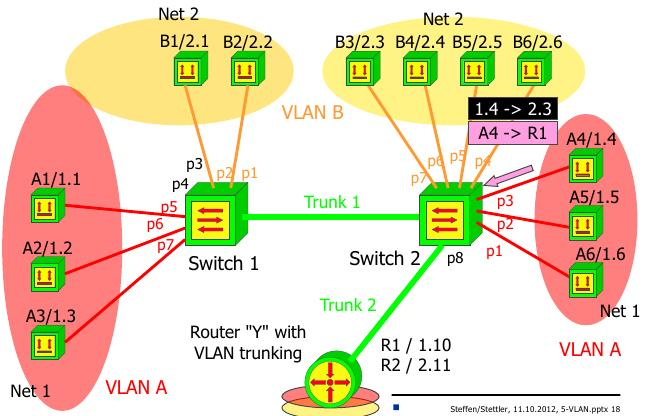
\includegraphics[width=\textwidth]{img/V5.6.jpg}
	\caption{Router mit Trunkport}
	\label{}
\end{figure}
\begin{figure}[H]
	\centering
	 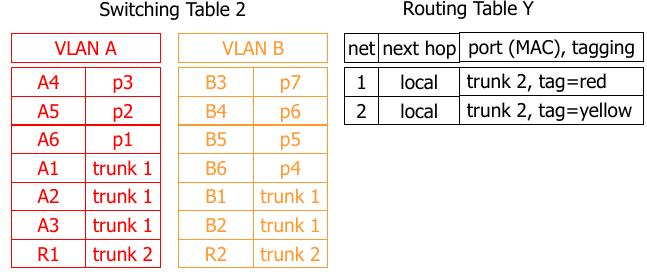
\includegraphics[width=\textwidth]{img/V5.7.jpg}
	\caption{Switching und Routing Table}
	\label{}
\end{figure}

\expl{Switch und VLAN's}{Switch auf Layer2 kann nie zwischen VLAN's vermitteln, auch wenn die Pakete beider VLAN's über diesen Layer laufen.}
\exam{Wissen, dass Switch keine Vermittlung zwischen VLAN's machen kann}

\se{Layer3 Switching}
\definition{Layer3 Switch}{Multiport Router, routing wird durch die Hardware abgehandelt (ASICs)}

\sse{VLAN Zuordnung}
Wie weis Switch, welcher Port zu welchem VLAN gehört?
\ul
	\li Basierend auf den Port (Hart festgelegt)
	\li Basierend auf die Mac Adresse (flexibel)
	\li Protokoll basiert (Eigene VLAN's für IP, IPX, Decnet, Appletalk, ...)
\ulE

\se{Spanning Tree und VLAN}
\begin{figure}[H]
	\centering
	 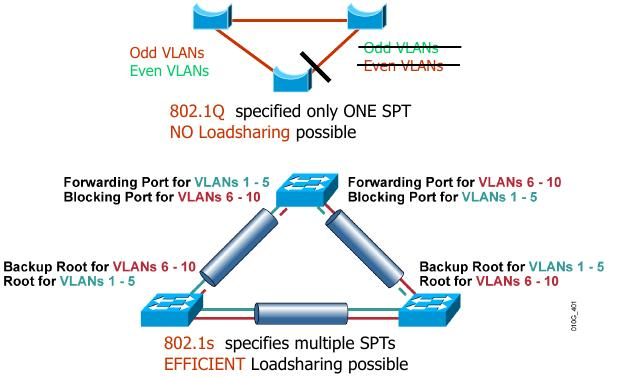
\includegraphics[width=\textwidth]{img/V5.8.jpg}
	\caption{Spanning Tree and VLANs, 802.1Q vs 802.1s}
	\label{}
\end{figure}
\ul
	\li Pro VLAN kann eine eigene Rootbridge definiert werden.
	\li 802.1s Erlaubt unterschiedliche SPanning Trees für unterschiedliche VLANs
\ulE
\definition{Layer3 Switch}{Gerät, dass einen Switchteil und einen Routerteil besitzt. Switchteil übernimmt Switchfunktionen und arbeitet mit Learning Table. Routingteil besitzt Routing Table, die konfiguriert wird.}

\expl{Router}{Router ist Software, analysiert Pakete ähnlich wie Wireshark, L3 Switch besitzt Router mit Hardware-Schalter (Switches)}

\se{Campus Design}
\sse{Flat Design}
\begin{figure}[H]
	\centering
	 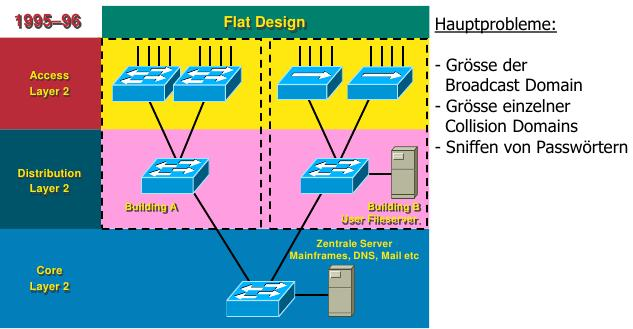
\includegraphics[width=\textwidth]{img/V5.9.jpg}
	\caption{Flat Design}
	\label{}
\end{figure}

\sse{Router-on-a-Stick Design}
\begin{figure}[H]
	\centering
	 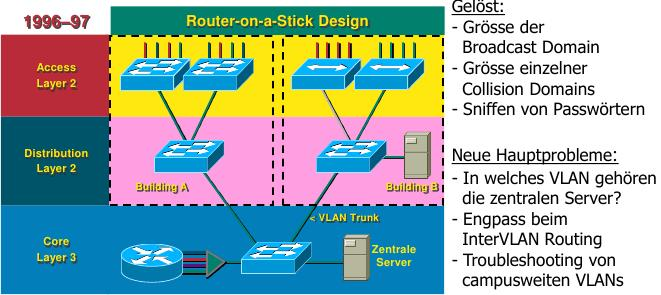
\includegraphics[width=\textwidth]{img/V5.10.jpg}
	\caption{Router-on-a-Stick Design}
	\label{}
\end{figure}

\sse{Collapsed Backbone Design}
\begin{figure}[H]
	\centering
	 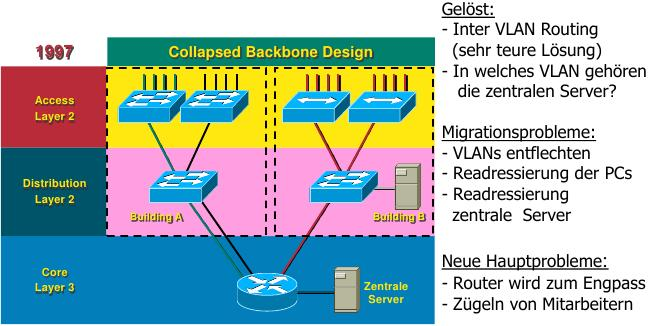
\includegraphics[width=\textwidth]{img/V5.11.jpg}
	\caption{Collapsed Backbone Design}
	\label{}
\end{figure}

\sse{L3 Distribution Design}
\begin{figure}[H]
	\centering
	 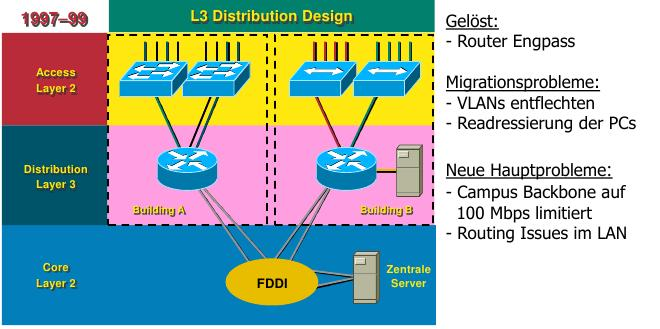
\includegraphics[width=\textwidth]{img/V5.12.jpg}
	\caption{L3 Distribution Design}
	\label{}
\end{figure}
\begin{figure}[H]
	\centering
	 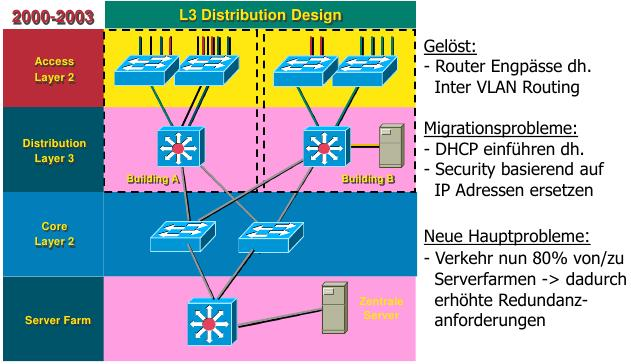
\includegraphics[width=\textwidth]{img/V5.13.jpg}
	\caption{L3 Distribution Design}
	\label{}
\end{figure}

\sse{MultiLayer Network Design (Today)}
\begin{figure}[H]
	\centering
	 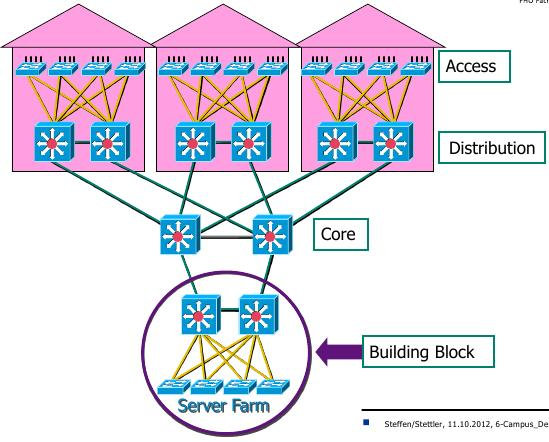
\includegraphics[width=\textwidth]{img/V5.14.jpg}
	\caption{MultiPayer Network Design}
	\label{}
\end{figure}

\se{Hot Standy Router Protocol Spanning Tree Design}
\begin{figure}[H]
	\centering
	 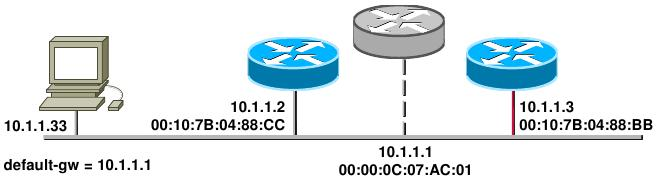
\includegraphics[width=\textwidth]{img/V5.15.jpg}
	\caption{HSRP—Hot Standby Router Protocol}
	\label{}
\end{figure}
\ul
	\li  Transparent failover of default router
 	\li “Phantom” router created
 	\li One router is active, responds to phantom L2 and L3 addresses
 	\li Others monitor and take over phantom addresses
\ulE
\begin{figure}[H]
	\centering
	 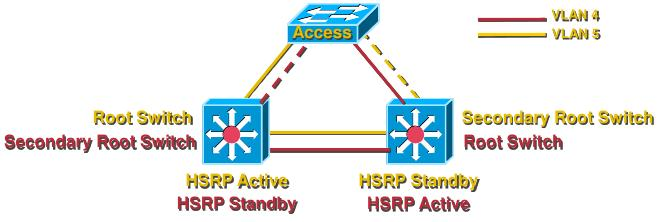
\includegraphics[width=\textwidth]{img/V5.16.jpg}
	\caption{Spanning Tree Design}
	\label{}
\end{figure}
\ul
	\li Spanning trees werden so aufgebaut, das alle Leitungen genutzt werden
	\li STPs verwenden unterschiedliche Root Switches
	\li Fällt einer aus, sucht STP automatisch neue Route
	\li Für Endhost sieht es aus, als sei es immer der gleiche Gateway, aber dahinter können unterschiedliche Geräte sein (Phantom Router).
\ulE

\sse{Oversubscription Guidelines}
\begin{figure}[H]
	\centering
	 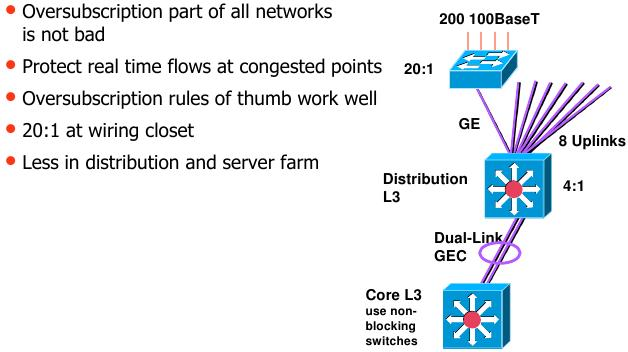
\includegraphics[width=\textwidth]{img/V5.17.jpg}
	\caption{Oversubscription Guidelines}
	\label{}
\end{figure}
\ul
	\li Nicht alle Hosts nutzen Kapazität aus. 
	\li Saugen Nutzer übermässig, stimmt die Rechnung nicht mehr \ra Kapazitätsprobleme
\ulE

\expl{VLAN Distanz}{VLAN über grössere Bereiche unkontrollierbar \ra Heute wird VLAN normalerweise an Gebäudegrenze terminiert und der Rest mit Routing gemacht (Projekt MA in andern Gebäuden)}

\expl{STP vs Routing}{Redundantes Routing auf Layer3 ist enorm Schnell beim Umschalten, wenn einer ausfällt. Viel schneller als STP.}

\sse{Core routing/switching}
\begin{figure}[H]
	\centering
	 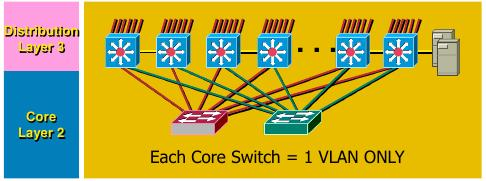
\includegraphics[width=\textwidth]{img/V5.18.jpg}
	\caption{Split Layer 2 Core}
	\label{}
\end{figure}

\begin{figure}[H]
	\centering
	 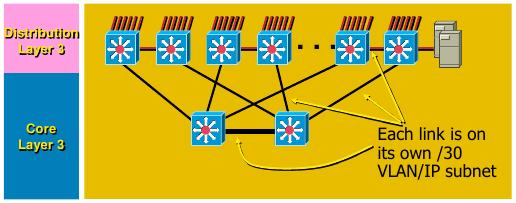
\includegraphics[width=\textwidth]{img/V5.19.jpg}
	\caption{Redundant Layer 3 Core v1}
	\label{}
\end{figure}

\begin{figure}[H]
	\centering
	 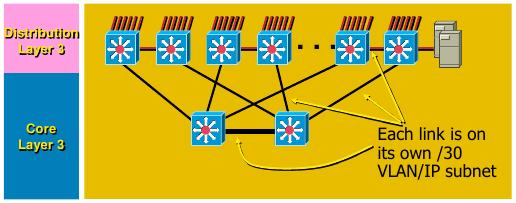
\includegraphics[width=\textwidth]{img/V5.19.jpg}
	\caption{Redundant Layer 3 Core v2}
	\label{}
\end{figure}


\ch{Wireless LAN}

\se{Architektur}
\begin{figure}[H]
	\centering
	 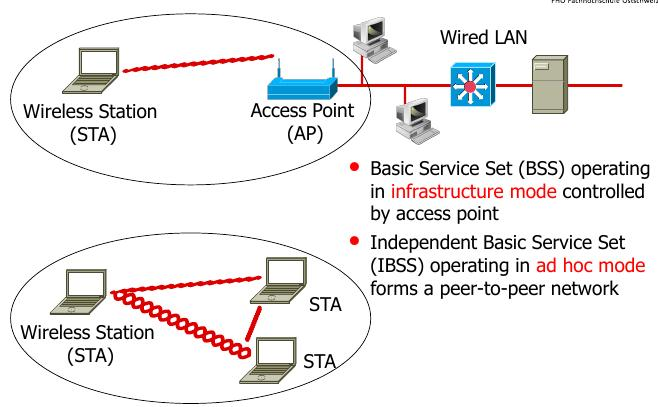
\includegraphics[width=\textwidth]{img/V6.1.jpg}
	\caption{WLAN Architektur}
	\label{}
\end{figure}
\definition{BSS}{Basisstation, auf welche sich die Clients verbinden}
\definition{IBSS}{Ad-Hock Netzwork direkt zwischen den Clients}

\sse{ESS}

\definition{ESS}{Extendes Service Set}
\definition{Quasi statisches Roaming}{Station wechselt Servicezone. Servicezonen sind über Distribution System verknüpft.}
\begin{figure}[H]
	\centering
	 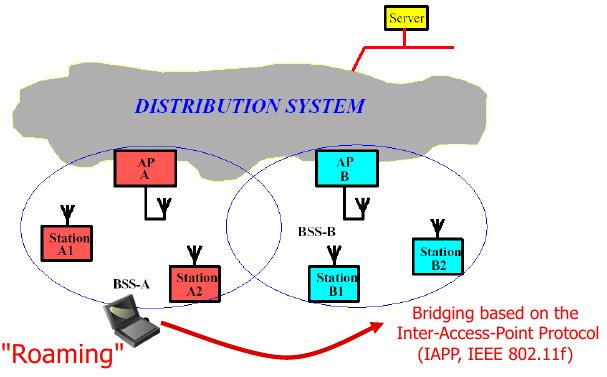
\includegraphics[width=\textwidth]{img/V6.2.jpg}
	\caption{Distribution System}
	\label{}
\end{figure}

\sse{Centralized Intelligence}
\begin{figure}[H]
	\centering
	 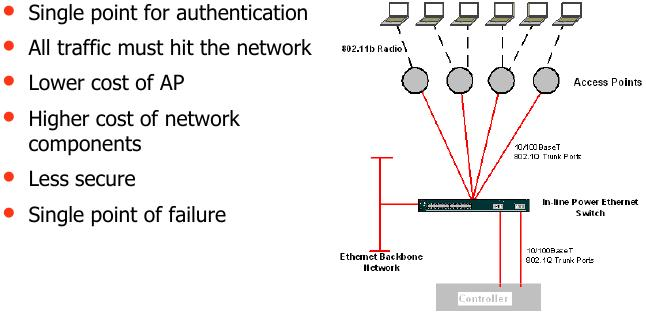
\includegraphics[width=\textwidth]{img/V6.3.jpg}
	\caption{Centralized Intelligence Architecture}
	\label{}
\end{figure}

\ul
	\li Accespoints sind über trunkports angeschlossen.
	\li Pakete sind getaggt.
	\li Vorteil: Accespoints sind günstig, werden über Power-over-Ethernet gespiesen.
	\li Controller ist "single point of failer"
\ulE

\sse{Synchronisation und Power Management}
\begin{figure}[H]
	\centering
	 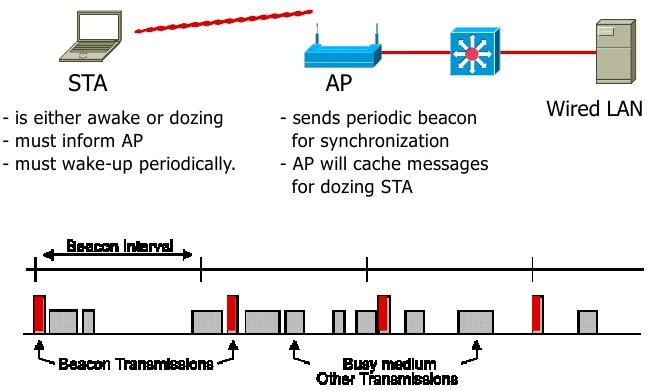
\includegraphics[width=\textwidth]{img/V6.4.jpg}
	\caption{Synchronisation und Power Management}
	\label{}
\end{figure}
\ul
	\li Beacon Frame sendet ESSID \ra Sicherheitsrisiko wenn ESSID Name und Adresse beinhaltet
	\li Powermanagement: Schläft und wächt zwischendurch (Paar Mal pro Sekunde) auf um zu überprüfen, ob neue Nachrichten eingetroffen sind.
	\li Beacon Frame kündigt an, ob während Sleep Phase des Clients etwas angekommen ist.
\ulE

\sse{Carrier Sense ultiple Access / Collision Avoidance}
\begin{figure}[H]
	\centering
	 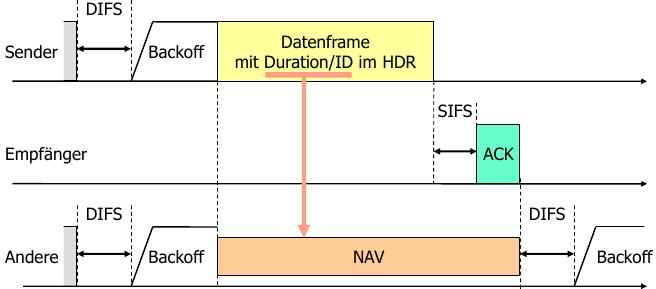
\includegraphics[width=\textwidth]{img/V6.5.jpg}
	\caption{CSMA / CA}
	\label{}
\end{figure}
\definition{NAV}{Network Allocation Vector}
\definition{DIFS}{Distributed Coordination Function Interframe Space}
\definition{SIFS}{Short Interframe Space}
\ul
	\li Signal wird viel schneller schwächer als bei Kabel
	\li Schwierig zu detektieren, ob Kanal belegt ist \ra Kollisionen werden soweit wie möglich vermieden
	\li in DIFS-Zeit darf niemand senden
	\li Exonentional Backoff: Zeitschlitze werden grösser
	\li Ablauf einer Phase:
		\ol
			\li MAC Frame wird zusammen mit Sendezeit übertragen
			\li Andern Empfänger wissen, dass sie in dieser Zeit gar nicht zu senden versuchen \ra setzen einen Counter (NAV) der runtergezählt werden und gehen schlafen
			\li SIFS: Kleine Pause, bevor Empfänger bestätigung sendet (ACK: Acknoledge).
			\li Kanal ist reserviert, bis Bestätigung durch ist
			\li Kommt bestätigung nicht, muss sich der Sender wieder einordnen und später erneut zu senden versuchen.
			\li Nach dem Difs Intervall beginnt das ganze von vorne
		\olE
	\li Acknowledge ist layer2 Bestätigung (zusätzlich zur TCP Bestätigung
\ulE
\important{Kanalbelegungsdauer wird übermittelt}

\sse{Hidden Terminal Problem}
\begin{figure}[H]
	\centering
	 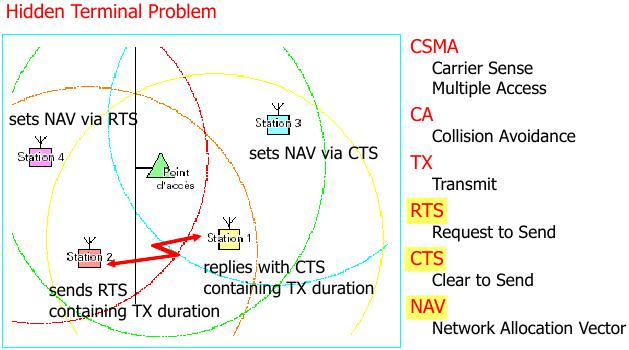
\includegraphics[width=\textwidth]{img/V6.6.jpg}
	\label{}
\end{figure}
\ul
	\li Nicht jeder Empfänger ist immer sichbar
	\li Empfangsradius ist in Praxis nicht kreisförmig!
	\li Station3 sieht Station2 nicht und funkt deshalb ev. Station1 rein
	\li Stationen höhren nur einen Teil der Kommunikation
	\li Stationen kriegen NAV nicht mit und beginnen zu senden
	\li RTS: Bei grossen Paketen wird zuerst einen Kurzen Austausch gemacht, in dem steht, wie lange die Station vor hat zu senden
	\li CTS: Empfänger bestätigt und damit bekommt z.B auch Station3 es mit
	\li Für kurze Pakete lohnt sich dieser Handshake nicht
	\li SIFS und DIFS überbrücken Zeitverzögerung, ansonsten sind Zeitverzögerungen kein Problem
\ulE
\begin{figure}[H]
	\centering
	 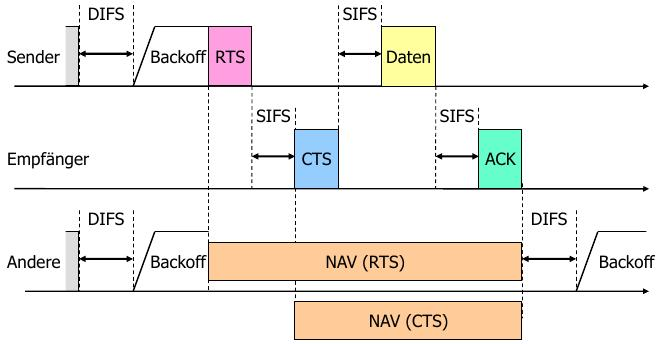
\includegraphics[width=\textwidth]{img/V6.7.jpg}
	\label{}
\end{figure}

\ch{WLAN Frequenzbänder}
\begin{figure}[H]
	\centering
	 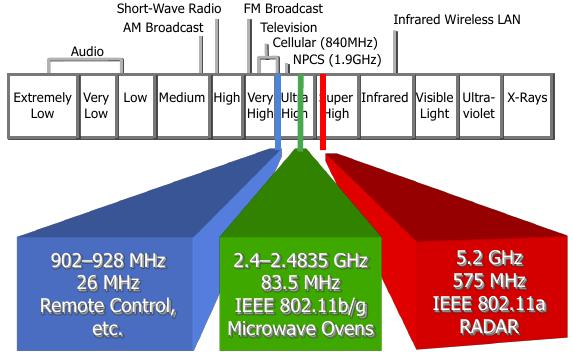
\includegraphics[width=\textwidth]{img/V6.8.jpg}
	 \caption{Vor allem "Schrottbänder" werden für WLAN verwendet}
	\label{}
\end{figure}

\ul
	\li 902-928: Bereich der Garagensteuerungen, etc.
	\li 2.4 - 2.4835: Industrial, Scientific und Medical Band (Mikrowellenöfen, etc) wurde für WLAN verwendet, weil es niemand will und keine Lizenz dafür notwendig wurde
	\li 5.2: Radar, Militär, unterdessen frei
	\li Im Moment werden viele Fernsehkanäle frei
\ulE

\sse{Kanalüberlappung}
\begin{figure}[H]
	\centering
	 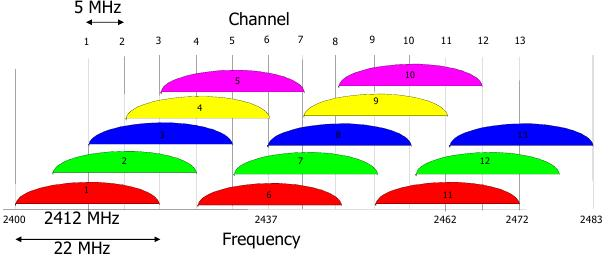
\includegraphics[width=\textwidth]{img/V6.9.jpg}
	 \caption{Vor allem "Schrottbänder" werden für WLAN verwendet}
	\label{}
\end{figure}
\ul
	\li Nur drei unabhängige Kanäle, weil sich die Kanäle überlappen
	\li Accespoints automatisch auf Kanal 1, 6 oder 11 eingestellt
	\li Kanal 6 ist der häufigste
	\li Kanal 12 nur in Europa, daher von vielen Accespoints nicht verwendet
	\li Zum Nachbarn leicht verschobene Kanäle wesentlich schlimmer, als komplette überlagerung \ra Kanäle 2,3 etc. nicht verwenden
	\li 
\ulE

\sse{Dynamic Frequency Selection DFS}
\ul
	\li Pflicht, um prioritäre Signale wie Militär nicht zu stören
	\li Accespoint sucht sich selbst einen möglichst freien Kanal
\ulE
\begin{figure}[H]
	\centering
	 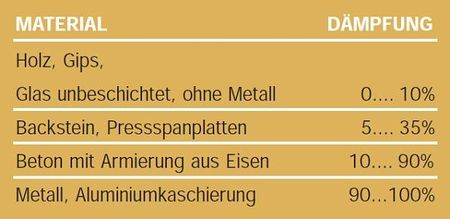
\includegraphics[width=\textwidth]{img/V6.10.jpg}
	 \caption{Signaldämpfung}
	\label{}
\end{figure}

\se{WLAN Datenraten}
\sse{IEEE 802.11n}
\begin{figure}[H]
	\centering
	 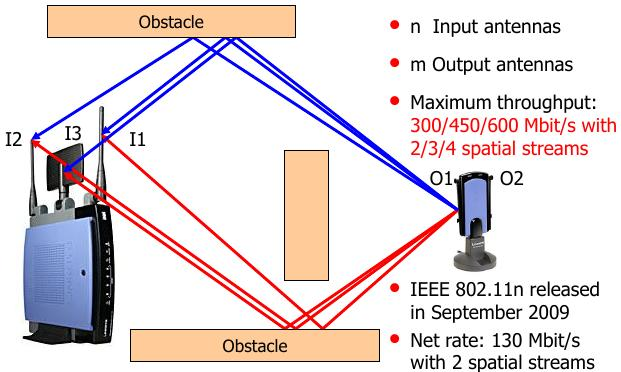
\includegraphics[width=\textwidth]{img/V6.11.jpg}
	 \caption{Reflexion}
	\label{}
\end{figure}

\ul
	\li Signal wird gespreizt, um Auslöschung durch doppelte Pfade zu vermindern
	\li Beim 802.11n Standard werden die Multiplen Pfade ausgenutzt
	\li Multiple In – Multiple Out (MIMO)
	\li mehrere Antennen verbessern das System
	\li Durchsatz wächst mit Anzahl Raumkanälen
	\li Reflexionen erwünscht, desto mehr, desto besser
\ulE

\sse{IEEE 802.11ac}
\expl{802.11ac}{Gigabit über die Luft}
\ul
	\li Kanäle bündeln, um Mehrkanalübertragung zu realisieren
	\li Viel mehr Antennen
	\li Bis zu 8 räumliche Ströme
	\li Mehrere Benutzer können gleichzeitig senden
\ulE

\se{WLAN Abdeckung und Reichweite}
\begin{figure}[H]
	\centering
	 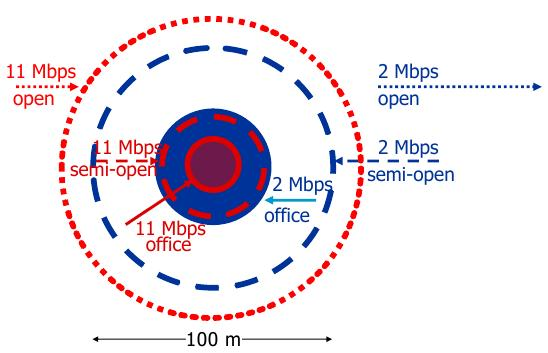
\includegraphics[width=\textwidth]{img/V6.12.jpg}
	 \caption{Maximum Distance Range}
	\label{}
\end{figure}

\ul
	\li Höhere Datenrate bedeutet immer kleinere Reichweite, ausnahme Verwendung paralleler Pfade
	\li 5GHZ Band: Dämpfung viel stärker, brauche viel mehr Accespoints
	\li Mikrowellengeräte stören im Umkreis 2m, Bandbreite bricht  um die Hälft ein
	\li Bluetooth stört WLAN auch
\ulE

\sse{Richtantennen}
\ul
	\li Signal bündeln und konzentriert bis zu einigen Kilometer übertragen
	\li Gesetzlich müsst Leistung reduziert werden
\ulE

\begin{figure}[H]
	\centering
	 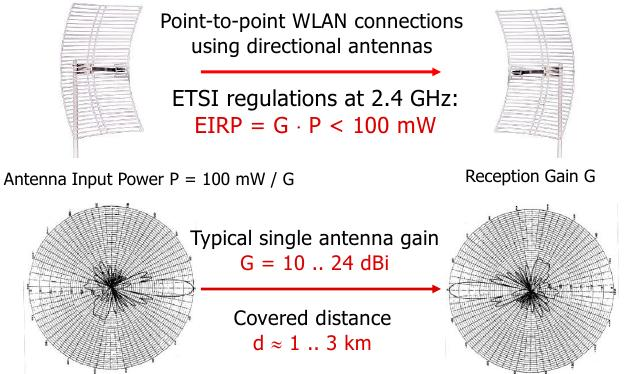
\includegraphics[width=\textwidth]{img/V6.13.jpg}
	 \caption{Richtantennen}
	\label{}
\end{figure}

\se{Schwachstellen und Attacken}
\ul
	\li Unbekannt, wer das Signal alles erhält
\ulE
\begin{figure}[H]
	\centering
	 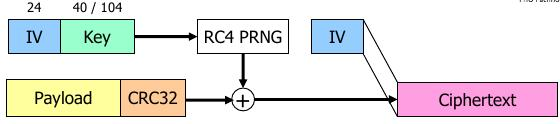
\includegraphics[width=\textwidth]{img/V6.14.jpg}
	\label{}
\end{figure}

\sse{WEP}
\expl{Was bringen MAC Filter?}{Verhindert Dummies, bringt aber sonst nichts weil sich die MAC Adresse von Karten mit einem Befehl ändern lässt.}
\ul
	\li Keine starke Verschlüsselung
	\li Aus den ersten Paar verschlüsselten Bits lässt sich auf den Schlüssel schliessen
\ulE
\important{WEP ist schwach und nutzlos}

\sse{WPA Wi-Fi Protectio Acces}
\ul
	\li WPA2: Verwendet nicht mehr RC4 Stream Cipher sondern AES
	\li Langes Passwort wichtig
	\li Personal Mode: Ein Passwort, Sicherheit steigt und fällt mit Passwort
	\li Bei professioneller Umgebung: Accespoint hat keine Keys, uncontrolled Ports dürfen alle ansprechen
	\li Authentisierung von Supplicant läuft über Authentication Server
	\li Server besitzt Zertifikat, um zu verhindern, dass jemand anderes einen eigenen AccesPoint aufsetzt und Passwörter snift
	\li Authenticator und Supplicant erhalten Schlüssel von Authentication Server
	\li Passwort wird über SSL Tunnel übertragen
\ulE

\begin{figure}[H]
	\centering
	 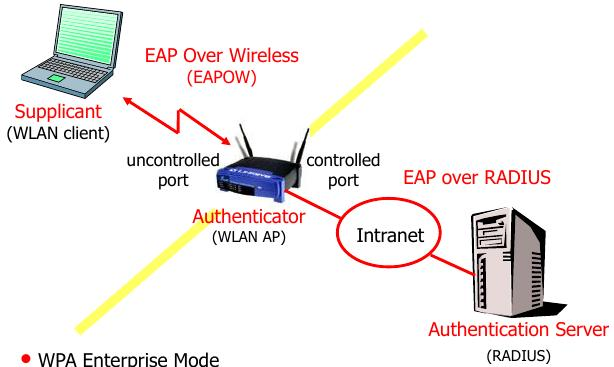
\includegraphics[width=\textwidth]{img/V6.15.jpg}
	\label{}
\end{figure}

\se{Pegelplan}
\begin{figure}[H]
	\centering
	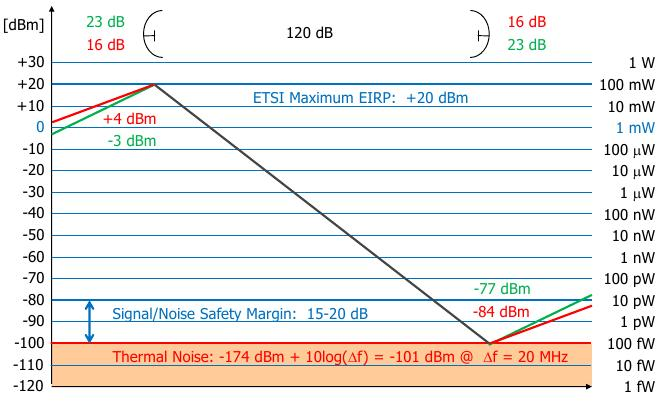
\includegraphics[width=\textwidth]{img/V7.1.jpg}
	\caption{Pegelplan WLAN-Richtstreke}
	\label{}
\end{figure}

\ul
	\li Rauschen aufgrund Feuchtigkeit im Raum (Thermal Noise)
	$Rauschen = -174dBm + 10log(Pegel)$
	\li Wenn 15-20dBm Abstand zu Rauschen ist Fehlerrate enorm klein ($10^-12$)
	\li Effektiver Sendepegel bei 23dB -3dB, weil Gesetzgeber 1mW als maximale Leistung vorschreibt.
	\li Links der Antenne: Bündelung (steigende Linie)
\ulE


\ch{DSL}
\definition{DSL}{Digital Subscrier Line}
\begin{figure}[H]
	\centering
	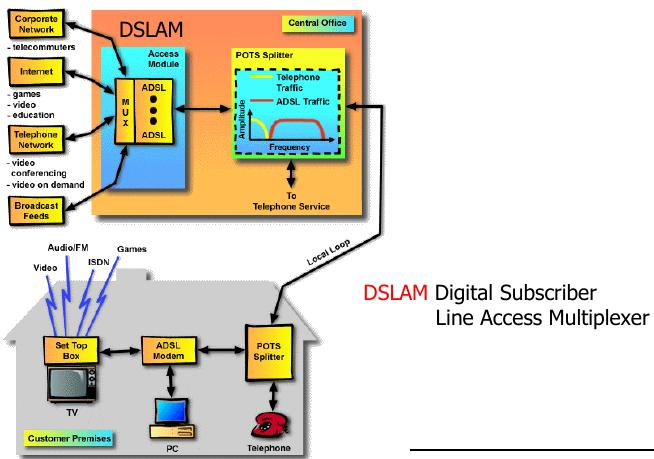
\includegraphics[width=\textwidth]{img/V7.2.jpg}
	\caption{}
	\label{}
\end{figure}

\ul
	\li Untere kHZ Bereich wird weiterhin für Telefon verwendet, Oberer Bereich für ADSL
	\li Frequenzweiche trennt Telefon und Daten, damit das menschl. Ohr die Daten nicht höhrt.
	\li Telefonsignal wird beim Provider digitalisiert und intern digital übertragen
	\li Upload zu Download mindesten 1:5, oft sogar 1:10
	\li Höhere Datenrate verkleinert Distanz
\ulE

\begin{figure}[H]
	\centering
	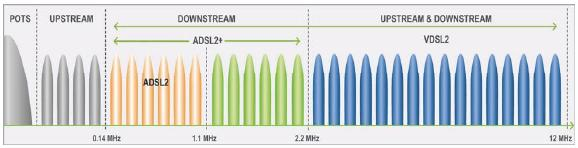
\includegraphics[width=\textwidth]{img/V7.3.jpg}
	\caption{ADSL/VDSL Kanalraster}
	\label{}
\end{figure}

\definition{POTS}{Plain old telefon}
\ul
	\li Nutzen von ganz vielen parallelen Modems
	\li Jedes Modem belegt ein 4 kHZ Band
	\li 
\ulE

\begin{figure}[H]
	\centering
	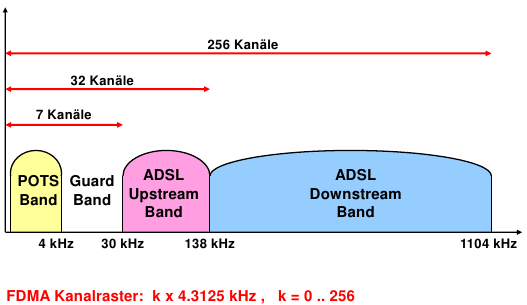
\includegraphics[width=\textwidth]{img/V7.4.jpg}
	\caption{ADSL mit POTS Splitter}
	\label{}
\end{figure}

\ul
	\li ISDN braucht viel mehr Bandbreite als POTS (80 bis 120 kHz)
\ulE

\sse{DMT}
\definition{DMT}{Discrete Multitone Verfahren}
\ul
	\li Zeigt Abstand zum Rauschen in jedem Kanal
	\li Sehr langsame Symbole, darum ADSL sehr robust
	 $fr = 4 kHz = 4k Band$
	$Tp = a/fr = 250us$
	\li Bis zu 15 Bit pro Symbol
	\li Kanäle sitzen genau auf Vielfachen der Grundfrequenz \ra Fouriersignal
\ulE

\begin{figure}[H]
	\centering
	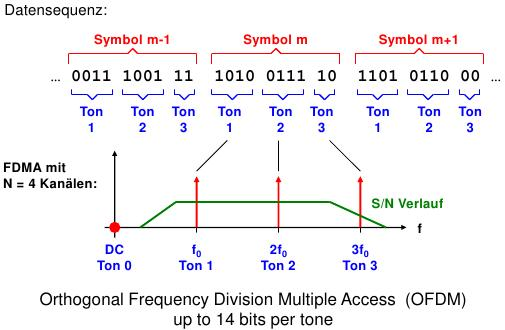
\includegraphics[width=\textwidth]{img/V7.5.jpg}
	\caption{}
	\label{}
\end{figure}

\definition{OFDM}{Orthogonal Frequency Division Multile Access (Sehr viele Modem Kanäle)}

\definition{QAM}{Quadratur Amplituden Modultaion, Horizontal die Modulation des Sinus, Vertikal des Cosinus}

\begin{figure}[H]
	\centering
	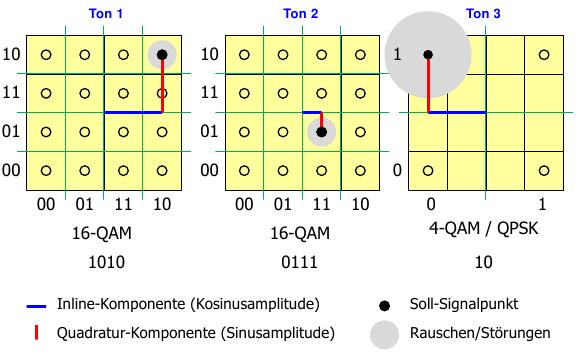
\includegraphics[width=\textwidth]{img/V7.6.jpg}
	\caption{}
	\label{}
\end{figure}

\ul
	\li ADSL Modem misst beim Verbindungsaufbau alle Kanäle durch und entscheidet für jeden Kanal, wie moduliert werden soll aufgrund der Dämpfung.
\ulE

\begin{figure}[H]
	\centering
	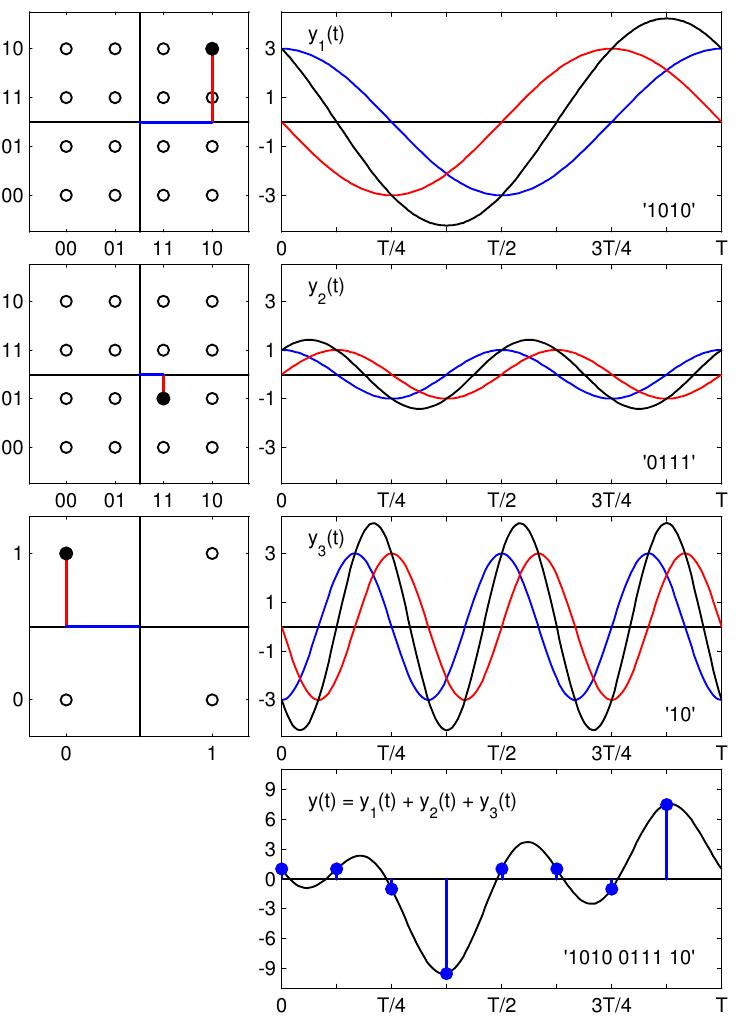
\includegraphics[width=\textwidth]{img/V7.7.jpg}
	\caption{OFDM}
	\label{}
\end{figure}

\begin{figure}[H]
	\centering
	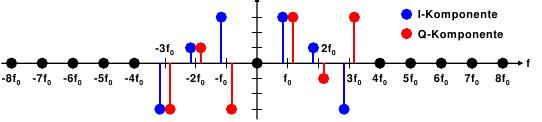
\includegraphics[width=\textwidth]{img/V7.8.jpg}
	\caption{OFDM mit 4 Kanälen}
	\label{}
\end{figure}

\begin{figure}[H]
	\centering
	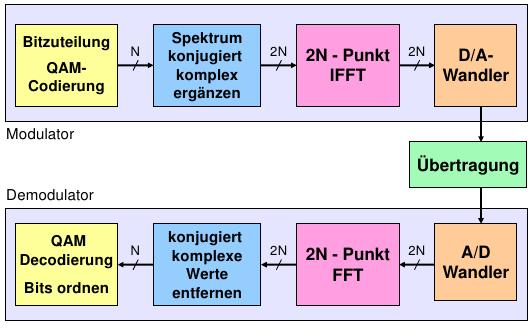
\includegraphics[width=\textwidth]{img/V7.9.jpg}
	\caption{OFDM Übetragungssystem}
	\label{}
\end{figure}


\ch{Internet Architektur}

\begin{figure}[H]
	\centering
	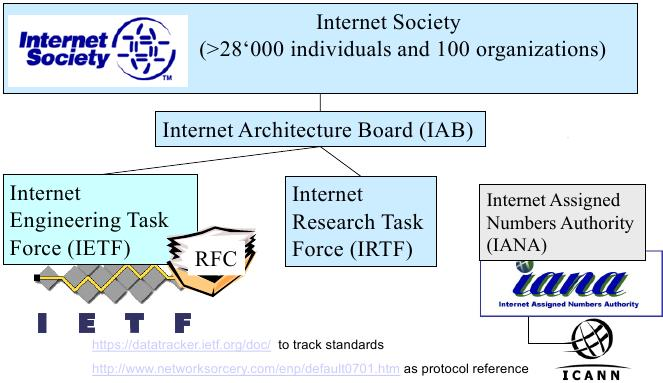
\includegraphics[width=0.75\textwidth]{img/V8.1.jpg}
	\caption{Internet Society ISOC}
	\label{}
\end{figure}

\begin{figure}[H]
	\centering
	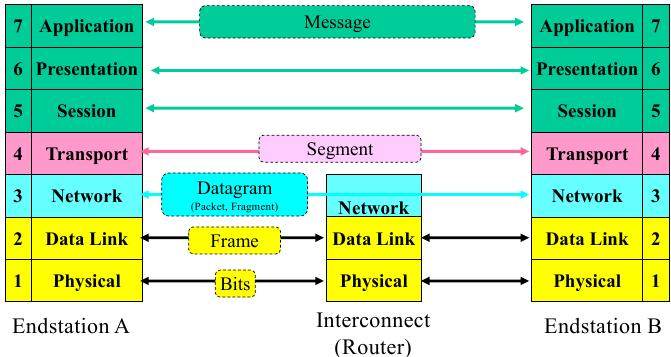
\includegraphics[width=0.75\textwidth]{img/V8.2.jpg}
	\caption{OSI Model}
	\label{}
\end{figure}
\exam{OSI Model mit Bezeichnungen können}

\begin{figure}[H]
	\centering
	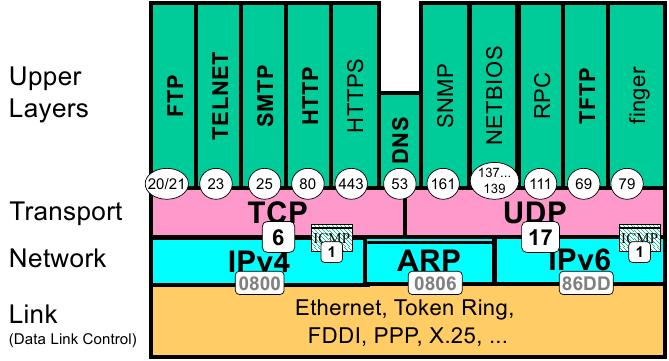
\includegraphics[width=0.75\textwidth]{img/V8.3.jpg}
	\caption{TCP/IP Protocol Stack}
	\label{}
\end{figure}

\begin{figure}[H]
	\centering
	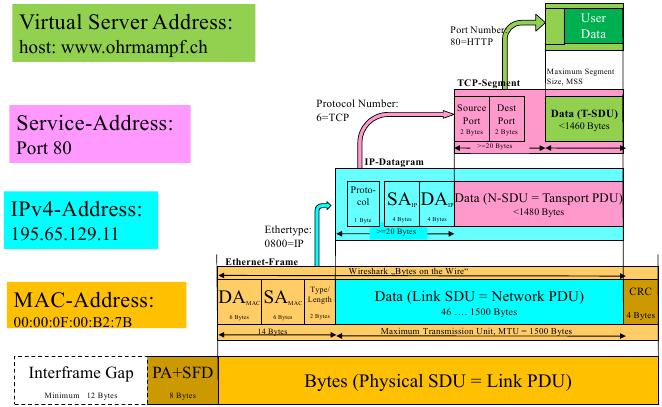
\includegraphics[width=0.75\textwidth]{img/V8.4.jpg}
	\caption{Internet Packet}
	\label{}
\end{figure}
\exam{Paketstruktur vorwärts und rückwärts erklären können}

\begin{figure}[H]
	\centering
	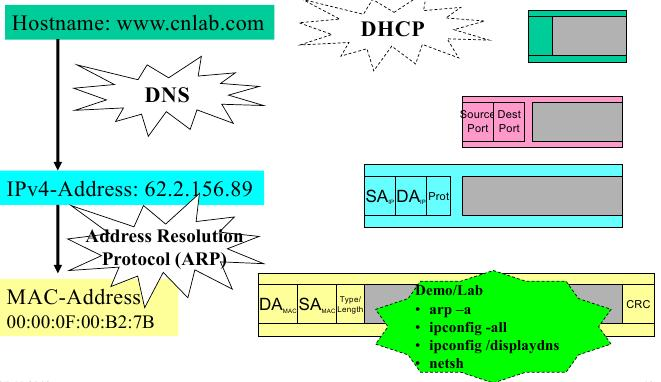
\includegraphics[width=0.75\textwidth]{img/V8.5.jpg}
	\caption{Address lookup}
	\label{}
\end{figure}
\definition{ARP}{Address Resolution Protocol}

\begin{figure}[H]
	\centering
	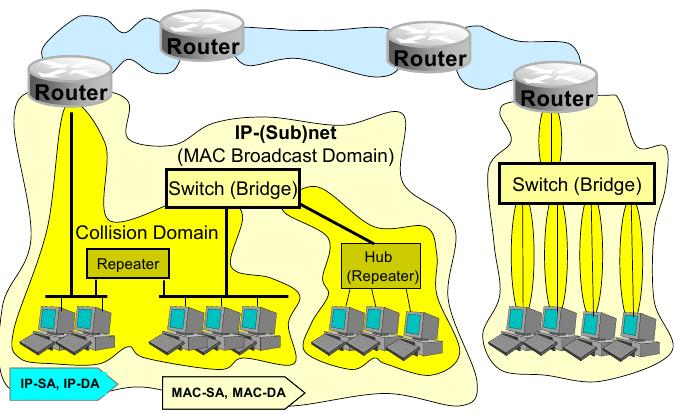
\includegraphics[width=0.75\textwidth]{img/V8.6.jpg}
	\caption{Internet Communication and Network Structuring}
	\label{}
\end{figure}

\expl{Woher weis Station, ob andere Station lokal oder entfernt ist?}{Anhand der Adresse}

\begin{figure}[H]
	\centering
	\includegraphics[width=0.75\textwidth]{img/V8.7.jpg}
	\caption{Network Structure}
	\label{}
\end{figure}

\expl{Tiers}{\newline
Tier1: erreichen einander direkt\newline
Tier2: brauchen Zwischenvermittler}

\begin{figure}[H]
	\centering
	\includegraphics[width=0.75\textwidth]{img/V8.8.jpg}
	\caption{Internet}
	\label{}
\end{figure}

\begin{figure}[H]
	\centering
	\includegraphics[width=0.75\textwidth]{img/V8.9.jpg}
	\caption{Autonomous Systems}
	\label{}
\end{figure}

\expl{Funktion Autonome Systeme}{
entscheidet, wer direkt miteinander verbunden ist. Pakete werden anhand der BorderNummer geleitet
}

\begin{figure}[H]
	\centering
	\includegraphics[width=0.75\textwidth]{img/V8.10.jpg}
	\caption{AS}
	\label{}
\end{figure}

\definition{AS}{Von einer Organisation administrierten Bereich}

\ul
	\li Stub-AS
		\ul
			\li Nur eine Verbindung zu anderen AS
		\ulE
	\li Multihomed AS
		\ul
			\li Mehrere Verbindungen zu anderen AS
			\li Leitet Verkehr anderer nicht weiter
		\ulE
	\li Transit AS
		\ul
			\li Verbindungen zu mehreren AS
			\li Leitet Verkehr anderer weiter
		\ulE
\ulE

\definition{Broadcast Domäne}{MAC Broadcast Domäne = IP Subnetz}


\ch{IP}
\ul
	\li Verbidungslose Kommunikation mit Endstelle (Nicht wie Telefon)
	\li Unzuverlässig, das Netzwerk kümmert sich nicht darum, wenn Pakete verloren gehen
\ulE

\exam{Rechnen können mit Subnetmasken und IP Adressen (~10Punkte). Binär -> Dez/Hex}
\expl{ARP und DNS}{DNS wandelt Domainnamen in IP Adressen, APR wandelt IP Adressen in MAC Adressen}

\se{IPv4}

\ul
	\li 32 Bit (4Byte)
	\li Reservierte Nummern:
		\ul
			\li non routable
			\li broadcast (all networks/hosts)
			\li Loopback (sich selbst)
			\li multicast (Bsp. Videoverteilung)
		\ulE
\ulE

\begin{figure}[H]
	\centering
	\includegraphics[width=0.75\textwidth]{img/V9.1.jpg}
	\caption{IPv4 Address and Net Mask}
	\label{}
\end{figure}

\ul
	\li IP Nummer und Angabe wie viel Bits für netzwerk und Host verwendet verden werden mit / getrennt: IP-Nummer/Anzahl Bits des Netzwerk Teils
\ulE

\begin{figure}[H]
	\centering
	\includegraphics[width=0.75\textwidth]{img/V9.2.jpg}
	\caption{Class based IP Address}
	\label{}
\end{figure}

\begin{figure}[H]
	\centering
	\includegraphics[width=0.75\textwidth]{img/V9.3.jpg}
	\caption{Subnetze}
	\label{}
\end{figure}

\examp{IP umrechnen}{Given the IP subnet 152.96.128.0/21\\
– Give the (sub)net address in binary form:\\
255.255.55.0\\
1001'1000 0110'0000 1000'0|000 0000'0000\\

– Note the IP address range for the hosts in this subnet (address of first and last host):\\
152.96.128.1 ... 152.96.135.254\\
1001 1000  0110 0000  1000 0|000 0000 0001 ... \\
1001 1000  0110 0000  1000 0|111 1111 1110\\

– Give the subnet mask in binary form:\\
11111111 11111111 11111000 00000000 \\

– Give the subnet mask in dotted decimal form:\\
255.255.249.0
}

\sse{Non Routable Adressen}
RFC 1597/1918: Unassigned Numbers (non-routable addresses,
Private address ranges, local addresses)\\
• 10.0.0.0/8 10.0.0.0 ... 10.255.255.255\\
• 172.16.0.0/12 172.16.0.0 ... 172.31.255.255\\
• 192.168.0.0/16 192.168.0.0 ... 192.168.255.255\\

\expl{ Berechnen Sie, wieviele non routable
Adressen man in einer Organisation maximal
haben kann.
– Class A = $2^24-2$
– Class B = $2^16$
– Class C = $2^?$
– Total =
}

\expl{Router}{Jeder Router hat zwei Adressen: Eine innere und äussere}

\begin{figure}[H]
	\centering
	\includegraphics[width=0.75\textwidth]{img/V9.4.jpg}
	\caption{IP Datagram}
	\label{}
\end{figure}

\begin{figure}[H]
	\centering
	\includegraphics[width=0.75\textwidth]{img/V9.5.jpg}
	\caption{TTL - Time-to-live}
	\label{}
\end{figure}

\sse{IP Options Field}
\ul
	\li 0...40 Byte gross
	\li Genutzt für Record Route \ra Jeder Router schreibt seine IP Adresse hinter die letzte ins Route Data field
	\li Wenn mehr als 9 sind die ersten 9 eingetragen, wenn mehr als 9 wird auch der Rückweg eingetragen
\ulE

\begin{figure}[H]
	\centering
	\includegraphics[width=0.75\textwidth]{img/V9.6.jpg}
	\caption{RR}
	\label{}
\end{figure}


\sse{Fragmentation}
\begin{figure}[H]
	\centering
	\includegraphics[width=0.75\textwidth]{img/V9.7.jpg}
	\caption{}
	\label{}
\end{figure}

\se{NAT - Network Address translation}
\ul
	\li interne Adressen in externe übersetzen
	\li Einige externe Adressen, viele interne Adressen
	\li Nur soviele gleichzeitige Verbindungen nach aussen möglich, wie echte Adressen am NAT Router vorhanden
\ulE

\begin{figure}[H]
	\centering
	\includegraphics[width=0.75\textwidth]{img/V9.8.jpg}
	\caption{}
	\label{}
\end{figure}


\se{PAT - Port Address translation}
\ul
	\li interne Ports werden in externe Adressen übersetzen
	\li unbegrenzt viele Ports, daher keine Beschränkung bei der Anzahl Verbindungen
	\li Unschön weil Layermix
\ulE

\begin{figure}[H]
	\centering
	\includegraphics[width=0.75\textwidth]{img/V10.1.jpg}
	\caption{}
	\label{}
\end{figure}


\ch{IPv6}
\se{Grundlagen}
\exam{IP Blöcke binär, hex und dezimal umrechnen können}
\sse{Vorteile}
\ul
	\li 128Bit (16Byte) Adressen
	\li mehrere Adress Hirarchien (verbessert Routing Effizienz)
	\li Nur der Sender kann Datagramms fragmentieren
	\li Optionale Daten werden im Extension Header übertragen (beliebige Länge)
	\li IPsec Header
	\li Flow Label zur Priorisierung von Datagrams
	\li ICMPv6 Router Solicitation und Router Advertisement geben immer den besten Default Gateway
\ulE

\sse{Adresstypen}
\ul
	\li Unicast (eindeutiges Ziel)
	\li Multicast (Alle Schnittstellen einer Multicast Gruppe)
	\li Anycast
\ulE

\sse{Adressaufbau}
\begin{figure}[H]
	\centering
	\includegraphics[width=0.75\textwidth]{img/V10.2.jpg}
	\caption{IPv6 Address}
	\label{}
\end{figure}

\ul
	\li Interface: einzelner Host
	\li Provider Bsp: Switch
\ulE

\begin{figure}[H]
	\centering
	\includegraphics[width=0.75\textwidth]{img/V10.3.jpg}
	\caption{}
	\label{}
\end{figure}

\sse{Beispiel IPv7 Interface ID}
\ol
	\li Ethernet MAC-Adresse: 58:55:ca:f3:e1:29 ff:fe einfügen: 58:55:ca: ff:fe :f3:e1:29
	\li Universal/Local Bit invertieren: 58=0101’1000 > 0101’1010 = 5a
	\li IPv6-Address: f080:5a55:caff:fef3:e129%en0 prefixlen 64 scopeid 0x4
	\li Interface Identifier: 5a55:caff:fef3:e129
\olE

\sse{Address scopes}
\ul
	\li  link-local-address\\
– fe80::/10 (fe80... bis febf...)\\
– sollen von Routern nicht weitergeleitet werden
	\li site-local-address\\
– fec0::/10 (fec0... bis feff...)\\
– entspricht privaten IPv4-Adressen (z.B.
192.168.x.x)
– nur innerhalb der gleichen Organisation geroutet
	\li global-address\\
– weltweit gerouted

\ulE

\se{IPv6 Header Format}
\begin{figure}[H]
	\centering
	\includegraphics[width=0.75\textwidth]{img/V10.4.jpg}
	\caption{}
	\label{}
\end{figure}
\ul
	\li Headerlänge, weil Headerlänge nicht mehr fix
\ulE


\se{Übergang IPv4 - IPv6}
\ul
	\li DualStack
	\li Tunneling (Verpacken von IPv6 in IPv4 Paket)
	\li NAT-PT
\ulE

\begin{figure}[H]
	\centering
	\includegraphics[width=0.75\textwidth]{img/V10.5.jpg}
	\caption{Tunneling 6in4 und 4in6}
	\label{}
\end{figure}

\begin{figure}[H]
	\centering
	\includegraphics[width=0.75\textwidth]{img/V10.6.jpg}
	\caption{6in4-Tunneling}
	\label{}
\end{figure}

\sse{Teredo Tunnel}
\ul
	\li  benötigt ein Dual-Stack Interface
 	\li Verpackt IPv6 in IPv4/UDP und entpackt IPv6
aus IPv4/UDP
 	\li Microsoft Lösung
 	\li Verwendung von Teredo Relays
\ulE

\expl{CIDR}{Classless Inter-Domain Routing: Subnetmaske beliebig setzen}


\ch{ICMP}
\begin{figure}[H]
	\centering
	\includegraphics[width=0.75\textwidth]{img/V10.7.jpg}
	\caption{IP Datagram with ICMP payload}
	\label{}
\end{figure}

\definition{PING}{Packet InterNet Groper}

\begin{figure}[H]
	\centering
	\includegraphics[width=0.75\textwidth]{img/V10.8.jpg}
	\caption{ICMP Echo Request \& Reply}
	\label{}
\end{figure}

\ul
	\li ICMP \& NAT: ICMP hat kein Feld für Port nummer, verwendet dafür Identifier Field
	\li pathPing kann Strecken mit hohen Paketverlust identifizieren (meist Router mit überlaufendem Puffer)
\ulE


\ch{Transport Layer Protokolle}
\se{Grundlagen}
\begin{figure}[H]
	\centering
	\includegraphics[width=0.75\textwidth]{img/V11.1.jpg}
	\caption{}
	\label{}
\end{figure}

\sse{Sockets}
\ul
	\li Zugang zu den Prozesse vom oder zum Transport Layer
(mit TCP oder UDP) werden eindeutig identifiziert durch
Sockets
	\li Socket = IP address(es) + TCP or UDP Port number(s)
	\li UDP Socket
		\ul
			\li Empfänger demultiplexiert Segemente anhand 2-Number Socket
(destination IP address + destination port number)
			\li Es werden nur Empfangsbuffer benötigt (keine Sendbuffer)
		\ulE
	\li TCP Socket
		\ul
			\li Empfänger demultiplexiert Segemente anhand 4-Number Socket
(source and destination IP address and port number)
			\li Es werden Sende- und Empfangsbuffer benötigt
		\ulE
\ulE

\sse{Ports}
\ul
	\li Ports identifizieren Prozesse oder Anwendungen
	\li Portstypen: 
		\ul
			\li  Well Known Ports: 0 ... 1‘023
 			\li Registered Ports: 1‘024 ... 49‘151
 			\li Dynamic (ephemeral, private) Ports: 49‘152 ... 65‘535\\
 			gelten nur etwa 2min (kurzzeitig)
		\ulE
\ulE

\se{UDP - User Datagrammm Protocoll}
\ul
	\li 8 Byte Protokoll Header
	\li End-zu-End Protokoll
	\li Keine Überprüfung, ob Pakete wirklich ankommen
	\li Besitzt auch Checksumme, weil früher weiter unten auch andere Protokolle als IP ohne Checksum verwendet wurden
	\li Verbindungslose
	\li Keine Flusskontrolle
	\li Multicastpakete möglich
	\li Ansprechen der Anwendung (Port in Destination enthalten)
\ulE

\begin{figure}[H]
	\centering
	\includegraphics[width=0.75\textwidth]{img/V11.2.jpg}
	\caption{}
	\label{}
\end{figure}

\begin{figure}[H]
	\centering
	\includegraphics[width=0.75\textwidth]{img/V11.3.jpg}
	\caption{}
	\label{}
\end{figure}

\expl{UDP Socket}{UDP socket (application) is fully identified by 2-tuple
“Destination IP-Address” and “Destination Port”
}

\begin{figure}[H]
	\centering
	\includegraphics[width=0.75\textwidth]{img/V11.4.jpg}
	\caption{}
	\label{}
\end{figure}

\ul
	\li Connectionless transport layer protocol
	\li Only 8 Byte header needed
	\li Simply acts as sender and receiver of datagrams
	\li Interfaces to IP without flow control (fast delivery)
	\li No error-recovery
	\li Need only receive buffer
\ulE

\begin{figure}[H]
	\centering
	\includegraphics[width=0.75\textwidth]{img/V11.5.jpg}
	\caption{UDP Package}
	\label{}
\end{figure}

\expl{Ist Traceroute auch mit TCP möglich?}{Ja, weil es nur auf das "Time-to-Live" ankommt, welches eine Paketschicht tiefer liegt.}

\sse{UDP Demultiplex}
\expl{Paket \& Clientunterscheidung}{Verwenden zwei Clients den gleichen Service auf einem Server, kann der Server die Pakete der Clients nicht unterscheiden. Daher wird der Source-Port noch mitgesendet um den Client zu identifizieren.}

\begin{figure}[H]
	\centering
	\includegraphics[width=0.75\textwidth]{img/V11.6.jpg}
	\caption{UDP Demultiplex}
	\label{}
\end{figure}


\se{TCP Transmissin Control Protocol}

\begin{figure}[H]
	\centering
	\includegraphics[width=0.75\textwidth]{img/V11.7.jpg}
	\caption{TCP RFC}
	\label{}
\end{figure}

\exam{Long thin type und long fat type verstehen}

\ul
	\li Bytes werden nummeriert und Ankommen kontrolliert
	\li Verbindungbehaftete Kommunikation
	\li Zuverlässiger Bytestrom (Kontrolliert, ob alles gesendet und empfangen wird)
	\li Senden wie Empfänger benötigen Puffer
	\li Sockets sind 4-Tupel
\ulE

\begin{figure}[H]
	\centering
	\includegraphics[width=0.75\textwidth]{img/V11.8.jpg}
	\caption{}
	\label{}
\end{figure}

\begin{figure}[H]
	\centering
	\includegraphics[width=0.75\textwidth]{img/V11.9.jpg}
	\caption{TCP Puffer}
	\label{}
\end{figure}

\begin{figure}[H]
	\centering
	\includegraphics[width=0.75\textwidth]{img/V11.10.jpg}
	\caption{TCP Source+Destination}
	\label{}
\end{figure}

\sse{aktive Verbindung}
Upper Layer Protocol (ULP) requests TCP to connect to
a remote system and assigns a socket
assive connections (accept)


\sse{passive Verbindung}
Webserver wartet auf bestimmtem Port auf Verbindung

\sse{TCP Header}
\begin{figure}[H]
	\centering
	\includegraphics[width=0.75\textwidth]{img/V11.11.jpg}
	\caption{TCP Package}
	\label{}
\end{figure}

\sse{TCP Connection}
\ol
	\li Client sendet Paket mit Destination Port und initial Sequence Nummer und synchronize Flag (Verbindung öffnen)
	\li Empfänger (Server) antwortet, indem er seine Sequence Nummer und aknowledge (Verbindungsaufbaubestätigung) dem Client sendet.
	\li Client bestätigt, das er auch die Verbindung aufnehmen will.
	\li Daten werden übertragen. Sequenznummer: Initial Sequence Number+1
\olE
\begin{figure}[H]
	\centering
	\includegraphics[width=0.75\textwidth]{img/V11.12.jpg}
	\caption{}
	\label{}
\end{figure}

\sse{Connection Closing}
\ol
	\li Client sendet "Verbindung schliessen"
	\li Server bestätigt
	\li Server schliesst Anwendungen
	\li Client bestätigt Connection close
\olE
\begin{figure}[H]
	\centering
	\includegraphics[width=0.75\textwidth]{img/V11.13.jpg}
	\caption{}
	\label{}
\end{figure}

\sse{TCP Reliable Stream}
\ul
	\li Jedes Byte hat virtuelle nummer
	\li Erstes Segment enthält die ersten Bytes (8 hier nur Beispiel!)
	\li Zweites Paket: Erstes Byte wird mit 9 nummeriert
	\li Drittes Paket: Erstes Byte wird mit 17 nummeriert
\ulE
\begin{figure}[H]
	\centering
	\includegraphics[width=0.75\textwidth]{img/V11.14.jpg}
	\caption{}
	\label{}
\end{figure}

\sss{TCP Reliable Stream Scknowledge}
\begin{figure}[H]
	\centering
	\includegraphics[width=0.75\textwidth]{img/V11.15.jpg}
	\caption{}
	\label{}
\end{figure}

\ul
	\li Paket muss mindestens für Rount-Trip Zeit im Puffer behalten werden
	\li Als Acknowledge wird die Nummer des nächsten Bytes gesendet
	\li Wenn Paket nach timeout nicht angekommen ist, wird es erneut gesendet
	\li Timeout liegt im Bereich 3s
\ulE
\examp{Datenrate}{Roundtrip mit 8ms und 1460 Byte Paketen: 1240 kb/s ~1.5MB/s}

\begin{figure}[H]
	\centering
	\includegraphics[width=0.75\textwidth]{img/V11.16.jpg}
	\caption{}
	\label{}
\end{figure}
\begin{figure}[H]
	\centering
	\includegraphics[width=0.75\textwidth]{img/V11.18.jpg}
	\caption{}
	\label{}
\end{figure}

\sss{Kummulativer Acknowledge}
Höchste, vollständig empfangene Bytenummer wird gesendet
\begin{figure}[H]
	\centering
	\includegraphics[width=0.75\textwidth]{img/V11.17.jpg}
	\caption{}
	\label{}
\end{figure}

\sss{Window Size}
Soviele Pakete darf der Sender schicken, ohne dass er auf die Bestätigung warten muss.

\begin{figure}[H]
	\centering
	\includegraphics[width=0.75\textwidth]{img/V11.19.jpg}
	\caption{}
	\label{}
\end{figure}

\ol
	\li Sender meldet Window Size 16 Byte.
	\li Empfänger bestätigt Erste 8 Byte
	\li Sender darf sliding Window nur um 8 Byte verschieben
	\li 
\olE

Sliding Window: Schiebt sliding Window um die Pakete, für die er Acknowledge erhalten hat.

\sss{Maximal mögliche Bandbreite bei best. Window Size}
Max. 1 Window-Size pro Round Trip.
\begin{figure}[H]
	\centering
	\includegraphics[width=0.75\textwidth]{img/V11.20.jpg}
	\caption{Time · Bandwidth Problem:
Increase Rwin}
	\label{}
\end{figure}

\begin{figure}[H]
	\centering
	\includegraphics[width=0.75\textwidth]{img/V11.21.jpg}
	\caption{Time · Bandwidth Problem:
Use Parallel Connections
}
	\label{}
\end{figure}






\end{document}
